\documentclass[tikz]{standalone}
\usepackage{pgfplots}
\usepackage{amsmath}
\usepackage{xcolor}
\usetikzlibrary{calc}
\definecolor{brown}{HTML}{8a4e3d}
\definecolor{blue}{HTML}{6d9eeb}
\definecolor{gray}{HTML}{888888}
\definecolor{gold}{HTML}{ffd966}
\pgfplotsset{compat=1.18}

\begin{document}
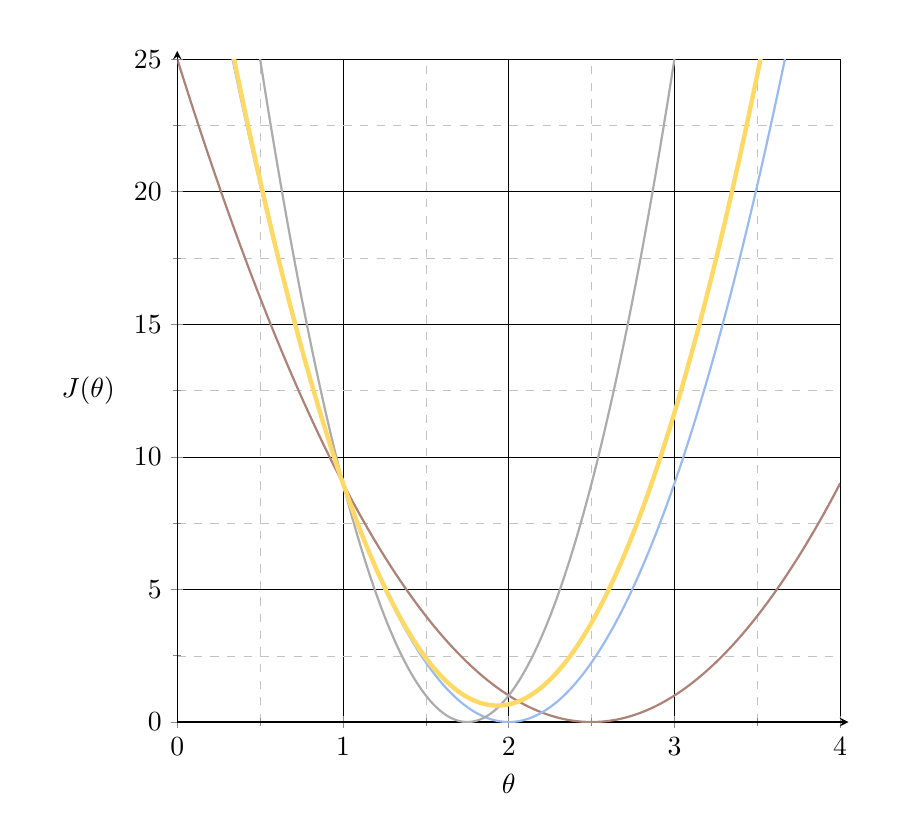
\begin{tikzpicture}
  \begin{axis}[
    axis lines=left,
    x axis line style={->,>=stealth, shorten >=-3pt},
    y axis line style={->,>=stealth, shorten >=-3pt},
    xlabel={\(\theta\)},
    ylabel={\(J(\theta)\)},
    ylabel style={rotate=-90},
    xmin=0, xmax=4,
    ymin=0, ymax=25,
    xtick={0,1,...,4},
    ytick={0,5,...,25},
    minor x tick num=1,
    minor y tick num=1,
    grid=both,
    major grid style={line width=0.2pt,draw=black},
    minor grid style={line width=0.1pt,draw=gray!50,dashed},
    width=10cm,
    height=10cm,
  ]
    % Individual curves (thinner)
    \addplot[domain=0:4, samples=200, thick, color=brown!70]
      {(2*x-5)^2};

    \addplot[domain=0:4, samples=200, thick, color=blue!70]
      {(3*x-6)^2};

    \addplot[domain=0:4, samples=200, thick, color=gray!70]
      {(4*x-7)^2};

    % Combined J(θ) = 1/3[(2θ-5)^2 + (3θ-6)^2 + (4θ-7)^2]
    \addplot[domain=0:4, samples=200, ultra thick, color=gold]
      {((2*x-5)^2 + (3*x-6)^2 + (4*x-7)^2)/3};

  \end{axis}
  \pgfresetboundingbox
  \useasboundingbox ([xshift=-19mm, yshift=-11mm]current axis.south west)
    rectangle ([xshift=4mm, yshift=4mm]current axis.north east);
\end{tikzpicture}
\end{document}
